\subsection{Functionality}
The main activity screen has two buttons for recovery mode, and hiding mode. There is also a help option that will take the user through a tutorial
of how to perform the recovery or hiding of their seed. This tutorial is aimed at making the user experience simple and helpful for the user. It starts
as default turned off so not to bother a user who has already used it before.

\begin{figure}[H]
	\centering
  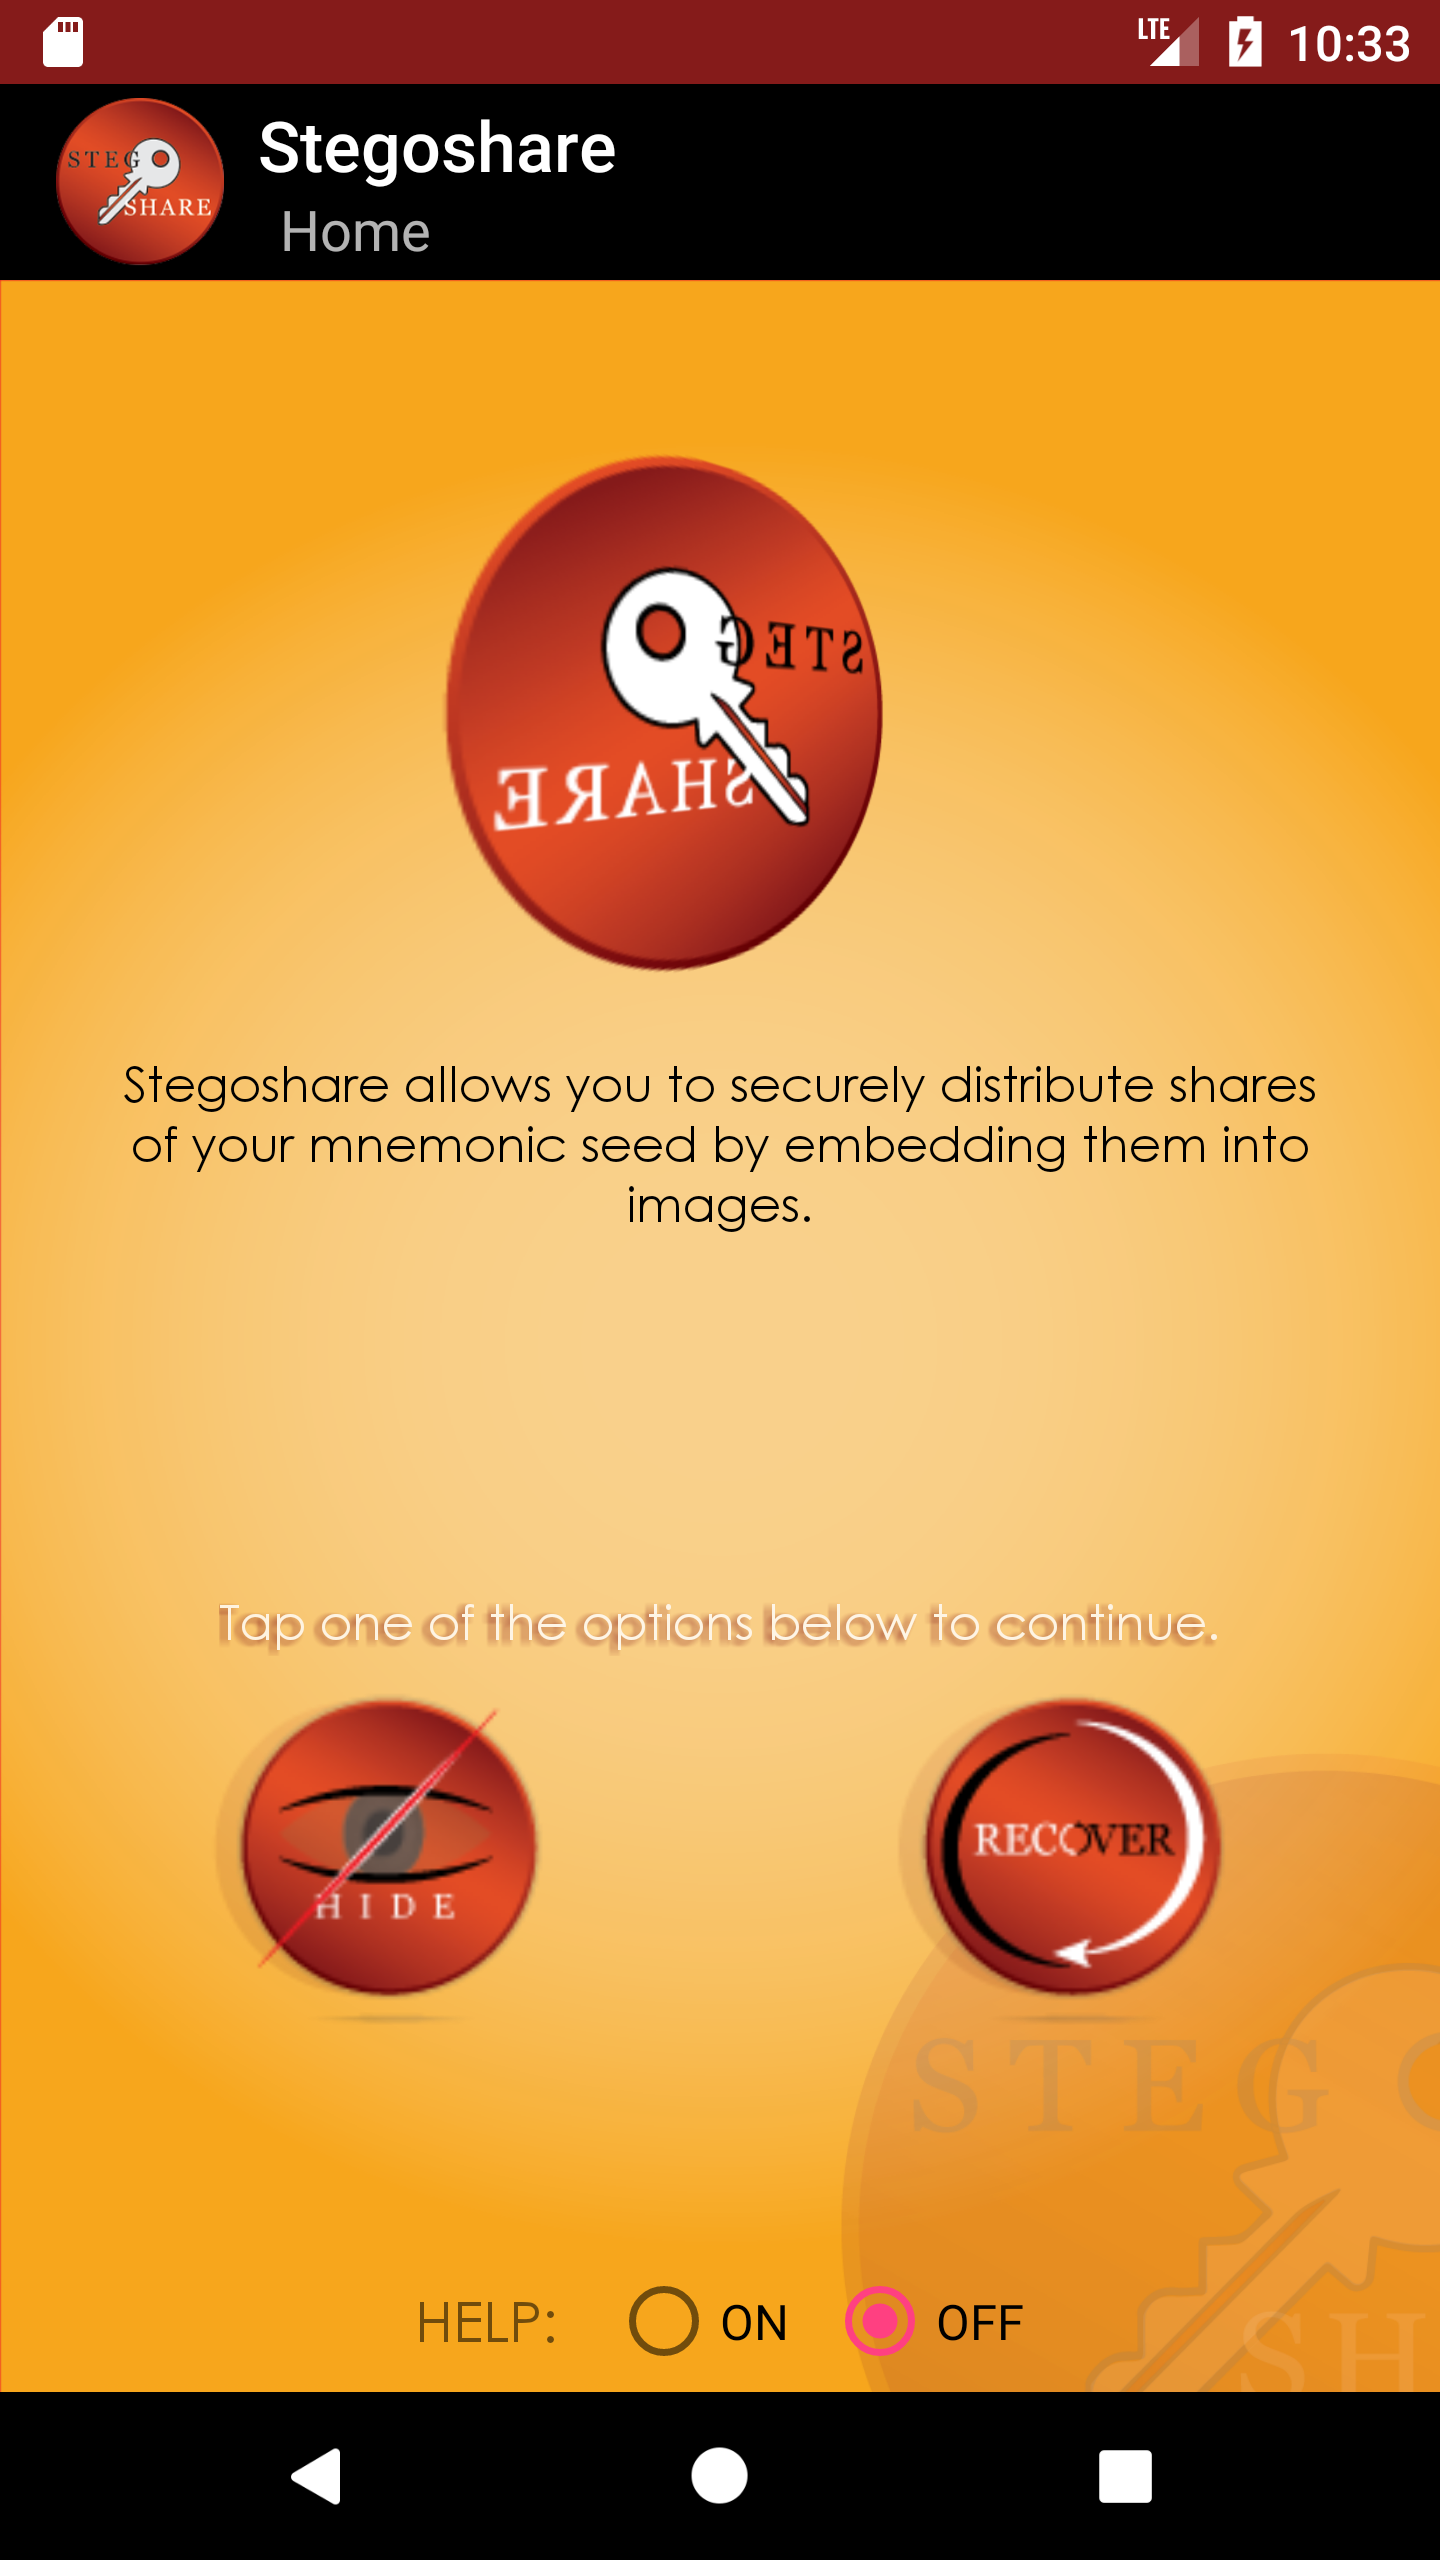
\includegraphics[scale = 0.05]{main_activity.png}
	\caption{Main Activity of Stegoshare}
	\label{fig: Main activity}
\end{figure}

	If the user selects the hide button, the hiding activity begins. In this activity the user is prompted to choose: the number of words, the total number of shares or images,
	and the number of shares(or images) that the user will need to recover their original message. Once the enter the words, they will go to a new activity where they can see
	all of the words they entered, and make any changes if necessary. Otherwise they can hit next to be prompted on whether or not they would like to encrypt their shares inside of
	the images. They can select yes and enter a password, or no and move on to the next activity - SelectImagesActivity. In addition to moving on to the next activity the shares will be split into
	N parts where N was selected by the user. We also use a database that uses two tables. One of the tables stores date, hashOfList, hashOfPassword while the other stores the N shares stored in the following form: prime number , share , share number, m, n
	, and dateID. These entries are used later for checking whether the user chose to use a password as well as in case of the application crashing. The date was planned on being used to automatically delete data after a certain period of time, although
	this was ultimately not implemented.

SelectImagesActivity is the where the user can see their selected images. To work properly, its intent must include \url{user_selected_shares_n}. This is necessary because the activity contains the galleryButton, which executes openGallery() on click.
This function will check that the application was granted the \url{READ_EXTERNAL_STORAGE} permission and starts CustomPhotoGalleryActivity and waits for its result.
The intent for the gallery contains the extra “numberOfParts” which is equivalent to \url{user_selected_shares_n}. numberOfParts communicates to the gallery activity how many images must be selected.
Which the external storage permission, CustomPhotoGalleryActivity uses MediaStore to get the ids and paths of all the images on the phone and instantiates imageAdapter.
This custom adapter tracks the selected images using an array of booleans “thumbnailsselection”, which is used to manage the checkboxes. Every time an image is clicked, the checkbox’s state is toggled.
The adapter also generates thumbnails for the images using the function setBitmap. setBitmap also runs as an AsyncTask, so the images are generated in the background.


  Once the user selects their photos, if the number selected is equal to numberOfParts (which is tracked using an array of booleans), the paths to the selected images are serialized and added to an intent that goes to SelectImagesActivity.
  SelectImagesActivity’s onActivityResult function will generates bitmaps using the provided image paths and add them to a LinearLayout in the activity. If the user is satisfied with their selected images, they can press the nextButton, starts UploadImagesActivity using an intent that contains the paths to the selected images.
  If they are not happy with their selection, they can press the gallery button and select a new set.


	In UploadImagesActivity, the images are encoded with the secret shares in the encoding function. The shares are stored as hashOfList, prime number, share, share numnber, m, n. This information is needed for the decoding process. For the case of encryption it is same format, only the entire string
	is itself encrypted. For the user to recover the formatted string they will need to enter their password. Then, using imagesAdapter and the image paths, thumbnails are generated for the encoded images. When the user presses the upload button, the share function is executed. This function generates URIs for the selected images using FileProvider. FileProvider requires an authority, which was declares in the AndroidManifest.
FileProvider is a very powerful tool because it allows the application to provide other applications temporary access to files. Any applications configured to receive URIs of images are capable of receiving them from Stegoshare. Because of this, implementing API’s for specific applications such as Google Drive or Gmail would be a gratuitous endeavor; it does not provide any additional functionality—rather it would slow down the application and increase its size and complexity.
If either of those applications is installed on the phone, they can be used to upload the encoded images.Once the user is done, they can press the finish button. This generates an alert dialog warning that once they confirm they are finished, all their data will be deleted. This is a security measure to ensure that the secret shares are no longer available. Once confirmed, the database containing the shares and the encoded images are deleted. Lastly, the activity closes by launching MainActivity.

Alternatively, the user can select recover if they already have the images that they want to decode. When they select the recovery option they proceed similarly to how they did in the
hide activity image selection. They will upload the images that they want to decode, and hit confirm. The images will be decoded and the program will decide whether or not the images have any
information encoded in them. If stegoshare does not successfully find any information it will notify the user it was unsuccessful and give them the option to select images again.


\subsection{Concepts applied}
Our application used a few concepts from class including Asynchronous Task to create the images in the background and display a progress update to the user.

1. Motivation - what is it good for?

2. Your solution – what does your app do? what functions does it offer to the user?

3. How does it work – key components and their interaction

 - Describe the user interface of your system and how it makes the most common tasks easy and quick to accomplish

 - Describe the key components of your systems (e.g., activities, services, remote database) and how they interact

 - Describe the implementation of selected key components so that a knowledgeable app engineer could create a similar app with the provided information.
4. How did you organize work in your team? What concepts from class did you apply?
